\subsection{Bi-clustering of hidden layer weights}
Let $W \in \mathbb{R}^{C \times X \times Y \times F}$ denote the weights of a second or later convolutional layer. Similar to the first convolutional layer approximation, we rely on the low dimensional linear structure of learned weights in a trained convolutional network to find an efficient approximation. We decompose $W$ by considering a partition of the input features into $G$ equal sized clusters and a partition of the output features into $H$ equal sized clusters. Then, for a given input cluster, $g$, and output cluster, $h$, we approximate the weights corresponding to the input and output features in those clusters, $W_{g,h} \in \mathbb{R}^{\frac{C}{G} \times X \times Y \times \frac{F}{H}}$, with a rank K tensor, $\tilde{W}_{g,h}$.  

We cluster the input features by concatenating the spatial and output feature dimensions of $W$ and clustering the resulting $C$ vectors in $\mathbb{R}^{XYF}$. This clustering can be done using k-means or a more sophisticated subspace clustering algorithm. In our experiments we found that often k-means was sufficient. We clustered the output features in an analogous manner and completely independently of the input clustering. 

We approximate the weight tensor for a given pair of input and output clusters with a sum of separable rank 1 tensors as described in section 4.2. Specifically, we approximate $W_{g,h}$ as
\begin{equation*}
	\tilde{W}_{f,g} = \sum_{k=1}^{K} \alpha_{k,g,h} \otimes \beta_{k,g,h} \otimes \gamma_{k,g,h}
\end{equation*}
where $\alpha_{k,g,h} \in \mathbb{R}^{\frac{C}{G}}$, $\beta_{k,g,h} \in \mathbb{R}^{XY}$ and $\gamma_{k,g,h} \in \mathbb{R}^{\frac{F}{H}}$.

We do not attempt to extend the separability in the spatial dimensions in our experiments because we found the rank required for a good approximation in this case was not worth the savings that resulted from the separability. However, we found that enforcing separability in the spatial dimension results in comparable approximation results and so could be used to reduce the number of parameters further if space constraints are a particular issue. 

The convolution operation with the approximated weights can easily be computed in the standard way by using $\tilde{W}_f$ rather than $W$. However, we can exploit the separability of each of the rank 1 tensors in the approximation to more efficiently compute the output. For a given input and output cluster pair, and for a particular rank $k$, we can compute the result of convolving the input signal with the tensor $W_{g,h}$ in three steps
\begin{enumerate}
\item Linearly combine the $\frac{C}{G}$ input maps using the $\frac{C}{G}$ coefficients from $\alpha_{k, g, h}$
\item Apply the $XY$ filter weights (multiply and sum) from $\beta_{k,g,h}$
\item Multiply the resulting scalar with the $\frac{F}{H}$ coefficients from $\gamma_{k,g,h}$ producing the $\frac{F}{G}$ different outputs for each output filter in the cluster 
\end{enumerate}

To compute the final target value for an output filter one must simply sum the result of these steps over the $\frac{C}{G}$ input clusters and $K$ ranks.

\subsubsection{Complexity analysis}
By using the bi-clustering low rank approximation to the convolutional weights of a hidden layer, the target output can be computed with significantly fewer operations. The number of operations that will be required is a function of both the number of input and output clusters and the rank used to approximate the tensors. Table \ref{biclustering_ops} gives the number of operations required in the original and approximated convolutions as a function of $G$, $H$ and $K$. 

\begin{table}[h]
\tiny
\parbox{\linewidth}{
\centering
\begin{tabular}{cc}
\hline
Original & Approximated \\
\hline
$C X Y F N M \Delta^{-2}$  & $G H N M \Delta^{-2} K (X Y \frac{C}{G} + X Y + \frac{F}{H} )$ \\
\hline
\end{tabular}
\caption{Number of operations required to compute target output of hidden convolutional layer with original weights vs. bi-clustered rank K approximation.}
\label{biclustering_ops}
}
\end{table}

Figure \ref{biclustering_ops_pic} shows the relative reduction in operations for varying values of $G$, $H$ and $K$.

\begin{figure}[t]
\centering
\mbox{
	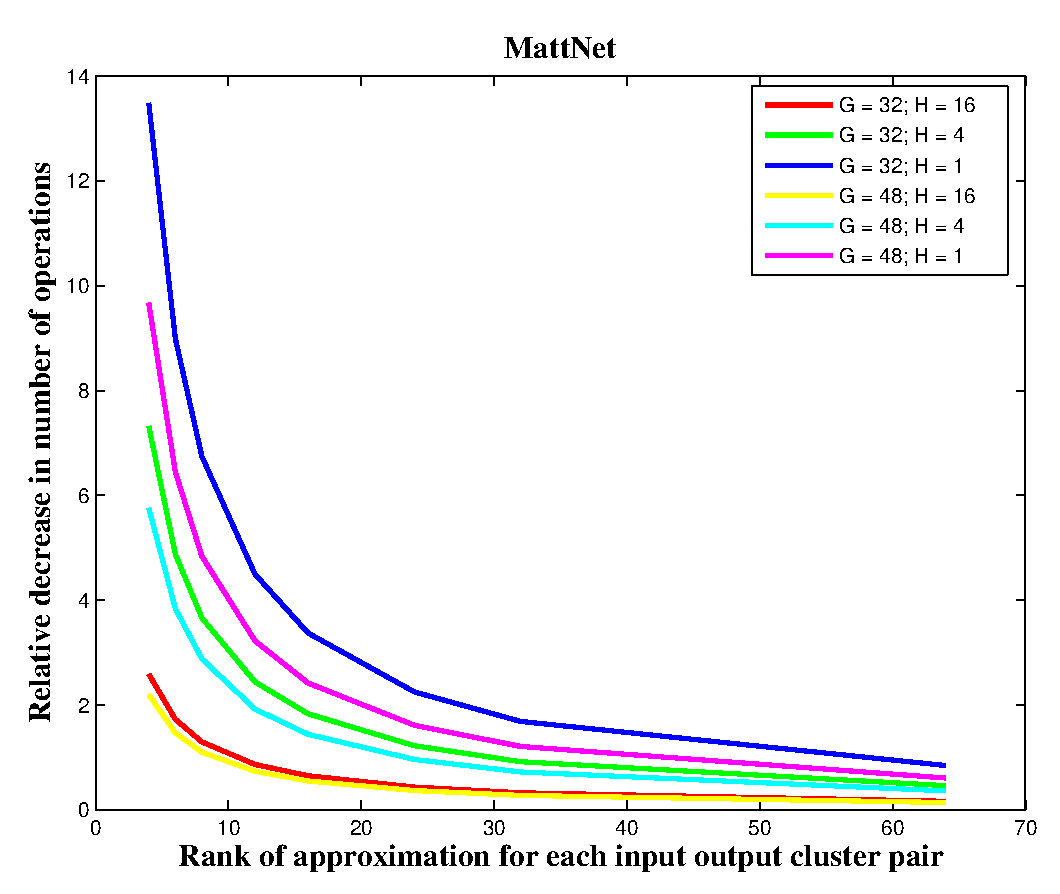
\includegraphics[width=0.75\linewidth]{img/bicluster_ranks_vs_numops_mattnet.eps} 
}
\label{biclustering_ops_pic}
\caption{Relative savings in number of operations required to compute target output of second convolutional layer of MattNet with the bi-clustered approximation and varying rank. Different input/output cluster sizes are plotted.}
\end{figure}


\subsubsection{Empirical performance}

\begin{figure}[t]
\centering
\mbox{
	\subfigure{
  		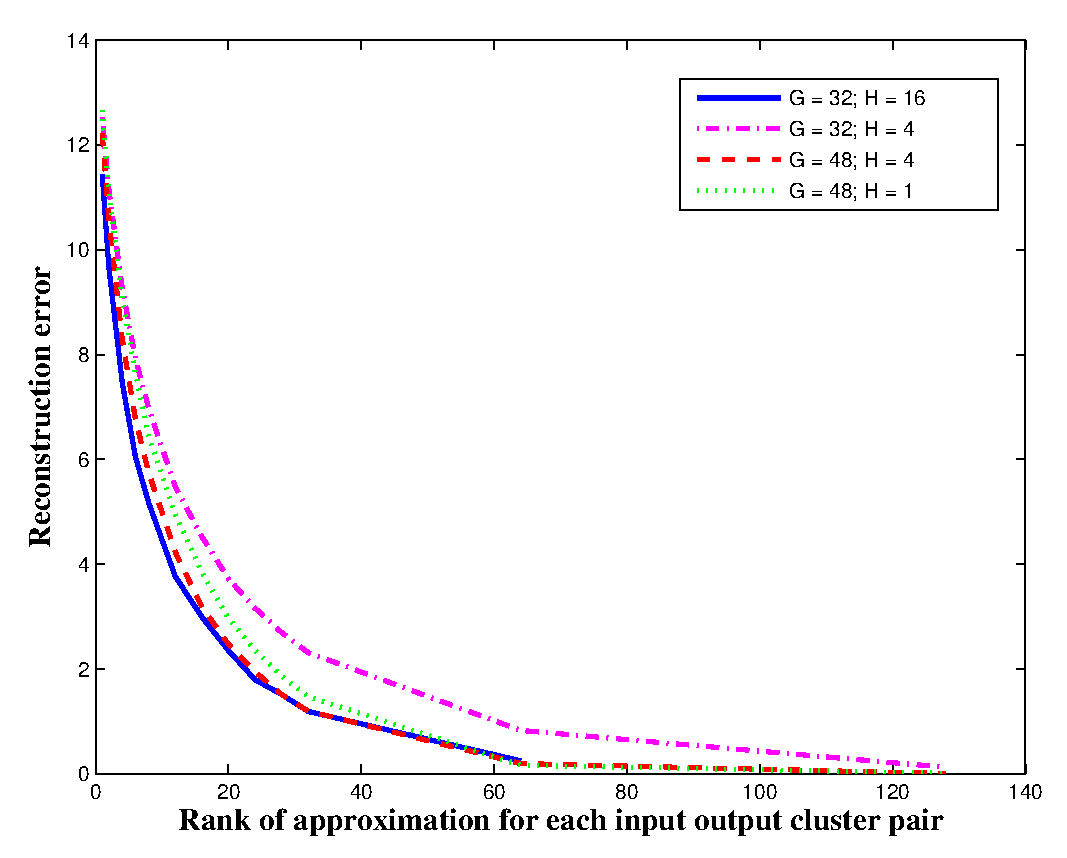
\includegraphics[width=0.48\linewidth]{img/layer2reconerror_vs_ranks.eps} 
	}
	\subfigure{
  		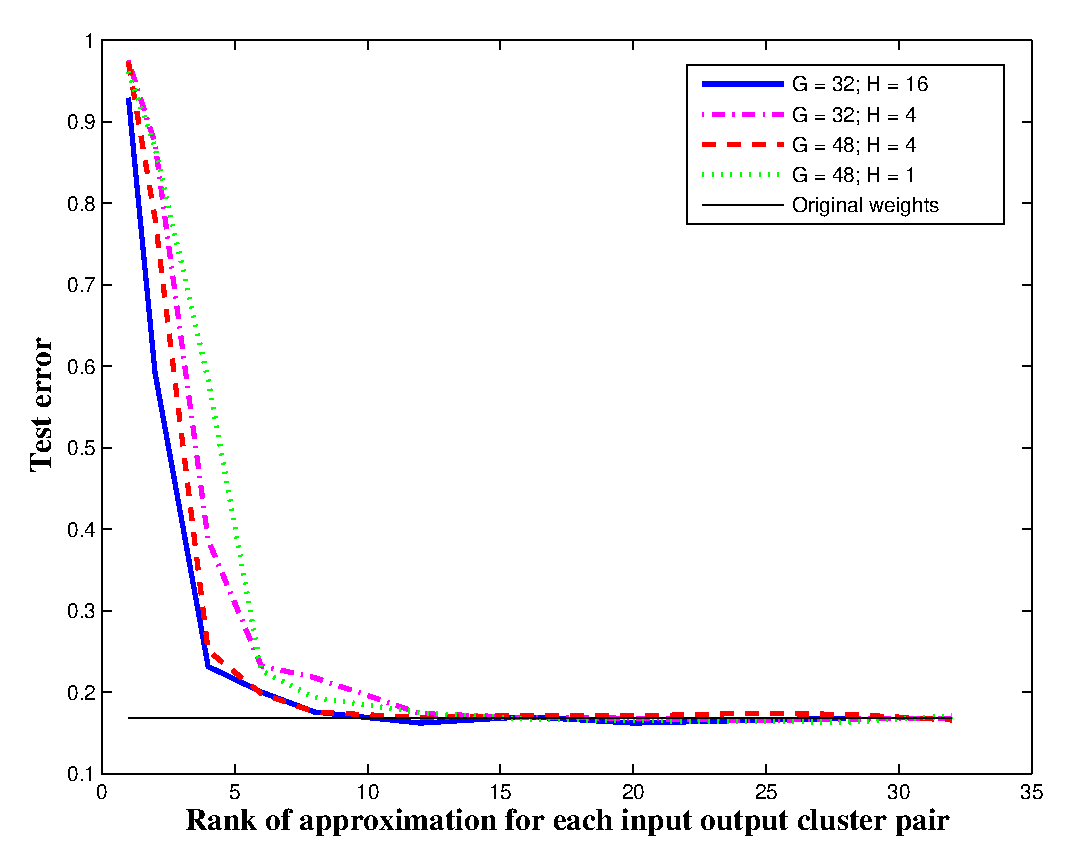
\includegraphics[width=0.48\linewidth]{img/layer2testerror_vs_ranks.eps} 
	}
}
\label{layer2recon_error_vs_rank}
\caption{Reconstruction error (left) and test error (right) for MattNet plotted against varying ranks used in the bi-clustering approximation for the second convolutional layer weights. Different input/output cluster sizes are plotted.}
\end{figure}
